\section{Responsible Research Statement}
\label{app:responsible_research}
\paragraph{Potential risks.}
\method{} is an analysis and evaluation framework, not a deployed agent-control system.
The main risks are over-interpreting outcome-informed graph roles as blind predictors of success, overfitting recovery policies to benchmark-specific traps, or using automated software-editing agents without human review.
We mitigate these risks by presenting the recovery pipeline as a local benchmark intervention on fired \swe{} states, using no gold patches or verified-test lists in the recovery note, reporting provider-specific behavior, and avoiding any deployment recommendation.

\paragraph{Artifacts, licenses, and intended use.}
We use access-controlled or provider-served research artifacts: the gated cx-cmu agent trajectory release on Hugging Face, the underlying benchmark suites and evaluation harnesses, and the three continuation models cited in \S\ref{sec:data} and \S\ref{sec:trap_intervention}.
The public card for the cx-cmu release gates file access behind contact sharing, and the public README does not list a separate dataset license or a detailed citation block.
We therefore cite the dataset card directly, treat the trajectories as access-controlled research material, and use them only for the analysis reported in this paper.
For the recovery study, GLM-5.1 and DeepSeek-V4-Pro are accessed through provider APIs under provider terms, while Qwen3.6-35B-A3B is run locally from Qwen-family weights whose public model card lists the Apache-2.0 license.
We do not redistribute raw trajectories, benchmark instances, source repositories, model weights, or API outputs.
Our intended use is research evaluation and process analysis of agent benchmarks, and any future sharing of derived artifacts would need to respect the access conditions of the source artifacts.

\paragraph{Privacy, content, and data handling.}
We do not collect new personal data, infer demographic attributes, or conduct user profiling.
The source artifacts consist of benchmark tasks, model-generated traces, tool outputs, repository paths, issue statements, and synthetic or benchmark-specific environment records.
We inspected the schema and representative examples for fields that directly name or identify people, and the analysis converts textual fields into canonicalized symbolic keys such as tool type, command class, observation pattern, file cue, and phase cue.
The paper reports aggregate statistics and illustrative benchmark snippets rather than raw private user conversations.

\paragraph{Computation and reproducibility.}
We do not train or fine-tune models.
Graph construction, annotation analysis, bootstrapping, and table generation use custom scripts over fixed symbolic signatures and fixed hyperparameters reported in \S\ref{sec:method} and Appendix~\ref{tab:hyperparams_full}.
The recovery experiment uses two API-served continuation providers (GLM-5.1 and DeepSeek-V4-Pro) and one locally hosted continuation model (Qwen3.6-35B-A3B).
Provider-side infrastructure for the API models is not observable to us, so we report model/provider names, data sizes, fired subsets, temperatures, top-$p$ values, confidence intervals, and permutation tests rather than provider GPU hours.
The locally hosted Qwen3.6-35B-A3B runs on a single NVIDIA H20 GPU, and the Qwen intervention sweep consumed approximately ten GPU-hours in total.

\paragraph{Human annotation.}
The graph-interpretability sanity checks use two internal annotators rather than crowdworkers or recruited human subjects.
The annotators were given task-level trajectory fragments and asked to judge within- vs. across-block similarity, articulation phase changes, and whether core/trap blocks correspond to productive progress or low-outcome exploration.
No external participants were recruited or paid, no annotator personal data were collected, and the annotation is used only as a sanity check for graph interpretability.
The full instruction text is in Appendix~\ref{app:annotation_guidelines}.

\paragraph{AI assistance.}
AI assistants were used for language polishing, LaTeX editing, patch preparation, and submission-checklist drafting.
The authors supplied the research ideas, experimental design, data analysis, and claims, and manually verified all citations, numerical results, and final text.
No AI assistant is treated as an author.


\section{Additional \method{} Details}
\label{app:details}

\subsection{Hyperparameters}
All graph and diffusion hyperparameters are fixed across benchmarks.

\begin{table}[h]
\centering
\small
\setlength{\tabcolsep}{5pt}
\begin{tabular}{ll}
\toprule
\textbf{Parameter} & \textbf{Value} \\
\midrule
Mutual-$k$NN $k$ & 6 \\
Edge-weight RBF scale $\sigma$ & 0.35 \\
Diffusion teleport $\alpha$ & 0.65 \\
Diffusion steps & 24 \\
Core quantile (top, $C_t$) & $0.75$ \\
Trap quantile (bottom of negative, $B_t$) & $0.25$ \\
Bootstrap resamples & $2{,}000$ \\
\bottomrule
\end{tabular}
\caption{Fixed hyperparameters used by \method{}.}
\label{tab:hyperparams_full}
\end{table}

\subsection{Rollout-Event Definitions}
\label{app:rollout_events}

The three rollout events in \S\ref{sec:profiles} are defined on the role overlays $(C_t,B_t)$.
For a rollout $r$ with compact primary-block sequence $b_{r,1:T_r}$ and visit set $V_r=\{b_{r,s}\}$:

\begin{align}
A_r &= \mathbf{1}[V_r\cap C_t\neq\emptyset], \label{eq:Ar}\\
E_r &= \mathbf{1}[V_r\cap B_t\neq\emptyset], \label{eq:Er}\\
R_r &= \mathbf{1}[\exists s<u:\, b_{r,s}\in B_t,\ b_{r,u}\in C_t]. \label{eq:Rr}
\end{align}

For binary benchmarks $y_r\in\{0,1\}$; for \mcp{} we use the per-task max-normalized continuous reward $y_r=\text{reward}_r/\max_{r'\in\mathcal{R}_t}\text{reward}_{r'}\in[0,1]$.

The model supply $S_{m,a}$ is the average over tasks of the task-centered cell residual:
\begin{align}
a_{m,t} &= \mathbb{E}_{r\in\mathcal{R}_{t,m}}[a_r], \nonumber\\
\tilde a_{m,t} &= a_{m,t}-\frac{1}{|M_t|}\sum_{m'\in M_t}a_{m',t}, \nonumber\\
S_{m,a} &= \mathbb{E}_t[\tilde a_{m,t}],
\end{align}
where $a\in\{A,E,R\}$.

The benchmark demand $D_{b,a}$ is the reward-weighted contrast over rollouts:
\begin{align}
D_{b,a}
&= \frac{\sum_{r\in b} w_r a_r}{\sum_{r\in b} w_r}
 - \frac{\sum_{r\in b} (1-w_r)a_r}{\sum_{r\in b} (1-w_r)}, \nonumber\\
w_r &= y_r.
\label{eq:Dba_app}
\end{align}
For binary $y_r$, $w_r$ is $0/1$ so Eq.~\ref{eq:Dba_app} reduces exactly to the mean-over-resolved minus mean-over-failed contrast.

\subsection{Axis Sign Sanity, Rollout Events}
\label{app:axis_sign_v2}

The three events are descriptive coordinates, not predictors, but they should still align with success in the expected direction across the corpus: high-outcome traffic should have larger $A$ and $R$ and smaller $E$ than low-outcome traffic.
Pooling all rollouts on the four binary splits and computing the unweighted contrast $\E_{y=1}[a_r] - \E_{y=0}[a_r]$ with $2{,}000$-bootstrap $95\%$ CIs, all three events have CIs that exclude zero in the expected direction (Table~\ref{tab:axis_sign_v2}).
Including \mcp{} under the continuous treatment gives the same qualitative pattern: positive Access, negative Trap, and small Repair.

\begin{table}[h]
\centering
\scriptsize
\setlength{\tabcolsep}{3pt}
\begin{tabular}{lcc}
\toprule
\textbf{Event} & \textbf{$\E_{y=1}-\E_{y=0}$} & \textbf{$95\%$ CI} \\
\midrule
Access ($A_r$)             & $+0.572$ & $[+0.544,\,+0.600]$ \\
Trap exposure ($E_r$)      & $-0.064$ & $[-0.091,\,-0.036]$ \\
Repair ($R_r$)             & $+0.040$ & $[+0.023,\,+0.057]$ \\
\midrule
All three sign-consistent  & \multicolumn{2}{c}{Yes} \\
\bottomrule
\end{tabular}
\caption{Rollout-event sign sanity on the four binary benchmarks (4,686 graph-valid binary rollout-event rows; 2,000-bootstrap $95\%$ CIs). All three main events shift in the expected direction at $p<0.05$.}
\label{tab:axis_sign_v2}
\end{table}

\subsection{Signature Ablation}
\label{app:signature_ablation}

We rebuild the pipeline on $150$ tasks under seven representation conditions.
The full signature has the largest model-separation statistic among non-degenerate representations and the broadest valid-task coverage; observation-only and no-phase variants remain useful, tool-only lowers separation while preserving broad coverage, and file-only, action-only, and random reassignment collapse coverage, with action-only yielding no stable separation estimate (Figure~\ref{fig:ablation}).

\begin{figure}[h]
\centering
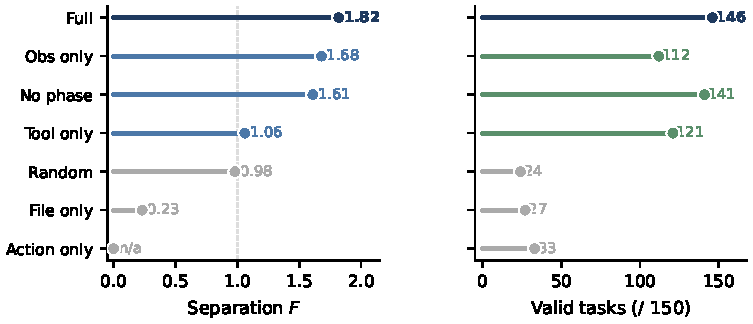
\includegraphics[width=\columnwidth]{figures/fig_appendix_ablation.pdf}
\caption{Signature ablation on $150$ tasks. Full signatures give the strongest model separation ($F=1.82$) and widest valid-task coverage ($146/150$); random, file-only, and action-only collapse coverage, and action-only yields no stable separation estimate.}
\label{fig:ablation}
\end{figure}

\subsection{Score Matrix and Reward Semantics}
\label{app:resolve}

The four binary-reward splits use the resolved/failed flag of each rollout.
For \mcp{}, the dataset provides a continuous multi-criteria reward; the main text uses the per-task max-normalized continuous reward $y_r=\text{reward}_r/\max_{r'\in\mathcal{R}_t}\text{reward}_{r'}$ throughout the reward field and benchmark-demand calculations.
A simple positive-reward threshold is near-saturated ($\sim\!97\%$ resolved across models), so we use the normalized continuous treatment instead; no threshold sweep is reported as a main result because the analysis avoids binarization altogether.

\subsection{Annotation Instructions}
\label{app:annotation_guidelines}

The graph-interpretability sanity checks used two internal annotators.
The annotators were shown de-identified task id, benchmark name, two or three consecutive trajectory fragments, and the graph-derived relation being checked; model identity and terminal outcome were hidden.
The instruction text was:

\begin{quote}
Read only the displayed action, observation, tool, file, and phase cues.
For a pair of steps, label them \emph{similar} if they represent the same local subtask, evidence-gathering mode, tool-use mode, or edit/debugging phase, even if the surface text differs; otherwise label them \emph{different}.
For an articulation crossing, label whether the second step marks a clear strategy or phase change relative to the first.
For a block, label the fragment as productive progress, exploration without convergence, repeated or stuck behavior, or unclear.
Do not infer model identity, do not use terminal success, and mark unclear when the displayed evidence is insufficient.
This annotation is for aggregate method validation only and should not identify any person or judge any human participant.
\end{quote}

No screenshots or additional risk disclaimers were used because the task was an internal, non-interactive annotation of already released agent traces.
The directional sanity-check $p$-values reported in \S\ref{sec:rq1} use one-sided alternatives matched to the stated hypotheses: within-BCC similarity $>$ across-BCC similarity, and core productive-progress rate $>$ trap productive-progress rate.

\subsection{Illustrative Annotation Examples}
\label{app:annotation_cases}

We show representative trajectory fragments from each of the three annotation tasks in \S\ref{sec:rq1}.
Tool arguments and observations are lightly trimmed for space.

\paragraph{BCC pair: within-block (similar).}
\swe{}, task \texttt{sympy-16886}.
Two steps from the same BCC block; the annotator labelled them \emph{similar}.

\smallskip\noindent\small
\begin{tabularx}{\linewidth}{@{}l@{\;\;}X@{}}
\textbf{A} & \texttt{view} \texttt{crypto/crypto.py:1500--1550} $\to$ Morse-code definitions \\[2pt]
\textbf{B} & \texttt{view} \texttt{crypto/crypto.py:500--600} $\to$ Vigen\`ere helpers \\
\end{tabularx}
\normalsize

\smallskip\noindent
Both steps view different sections of the same file, reflecting a single ``inspect source'' strategy.
The graph merges them because their key sets share the high-IDF key \texttt{FILE\_PATH:crypto/crypto.py}.

\paragraph{BCC pair: across-block (different).}
\swe{}, task \texttt{pytest-5773}.
Two steps from different BCC blocks; the annotator labelled them \emph{different}.

\smallskip\noindent\small
\begin{tabularx}{\linewidth}{@{}l@{\;\;}X@{}}
\textbf{A} & \texttt{bash}: \texttt{git show de6f.. | grep "python\_files"} $\to$ commit diff \\[2pt]
\textbf{B} & \texttt{str\_replace} on \texttt{\_pytest/python.py} $\to$ ``replaced'' \\
\end{tabularx}
\normalsize

\smallskip\noindent
Step~A inspects git history; Step~B edits source code.
Their key sets differ on tool, action type, command class, and observation pattern, so they land in separate blocks.

\paragraph{Articulation crossing: clear phase change.}
\terminal{}, task \texttt{processing-pipeline}.
Two steps immediately before and after an articulation point; the annotator labelled the crossing a \emph{clear phase change}.

\smallskip\noindent\small
\begin{tabularx}{\linewidth}{@{}l@{\;\;}X@{}}
\textbf{Before} & \texttt{read\_file} \texttt{collect\_data.sh} $\to$ shell script body \\[2pt]
\textbf{After} & \texttt{read\_file} \texttt{run\_pipeline.sh} $\to$ orchestration calling \texttt{collect}, \texttt{process}, \texttt{report} \\
\end{tabularx}
\normalsize

\smallskip\noindent
The rollout shifts from examining an individual component to the top-level orchestration wrapper.
The articulation point captures this strategy transition.

\paragraph{Core block: productive progress.}
\mcp{}, task \texttt{mcpbench\_10}.
Three consecutive steps from a block labelled \emph{core} by the diffusion field; the annotator judged the block \emph{productive progress}.

\smallskip\noindent\small
\begin{tabularx}{\linewidth}{@{}l@{\;\;}X@{}}
\textbf{1} & \texttt{MCP\_sum([10.3, 5.4, 8.2])} $\to$ \texttt{23.9} \\[2pt]
\textbf{2} & \texttt{MCP\_sum([52, 29, 43])} $\to$ \texttt{124} \\[2pt]
\textbf{3} & \texttt{MCP\_sum([52.2, 29.1, 43.2])} $\to$ \texttt{124.5} \\
\end{tabularx}
\normalsize

\smallskip\noindent
The rollout makes consistent, goal-directed MCP tool calls.
All observed visitors attain the task-local maximum normalized reward, placing the block firmly in the productive core.

\paragraph{Trap block: low-outcome exploration.}
\swe{}, task \texttt{django-14580}.
Three steps from a block labelled \emph{trap}; the annotator judged the block \emph{exploration without convergence}.

\smallskip\noindent\small
\begin{tabularx}{\linewidth}{@{}l@{\;\;}X@{}}
\textbf{1} & \texttt{view} \texttt{serializer.py:270--280} $\to$ \texttt{TypeSerializer} def \\[2pt]
\textbf{2} & \texttt{view} \texttt{serializer.py:170--190} $\to$ \texttt{functools} imports \\[2pt]
\textbf{3} & \texttt{view} \texttt{serializer.py:400--450} $\to$ (empty---file ends) \\
\end{tabularx}
\normalsize

\smallskip\noindent
The rollout reads scattered sections of the same file without converging on a fix.
Block purity is 0.125 (most visitors fail), placing it in the trap region.
Notably, 36\% of annotated trap blocks are labelled exploration rather than dead-end, consistent with the main-text observation that traps are low-outcome regions, not necessarily useless behavior.


\subsection{Robustness of Supply and Demand Profiles}
\label{app:sensitivity}

We report task-bootstrap CIs in the main text and additionally sweep the graph-role hyperparameters.
The qualitative signs used in the paper are stable under core-quantile, trap-quantile, Laplace-smoothing, diffusion, and mutual-$k$NN perturbations.
For \mcp{} under the continuous treatment, Access remains positive and Trap remains negative across the same perturbations, while Repair stays small.
Trap-averse conclusions for \mcp{} and \taub{} are stable across trap thresholds, and \swe{} remains the split with the strongest positive Repair demand across the baseline sweep.
The only borderline sign in the sweeps is \terminal{} Trap under the largest $k$NN setting, which is why the main text treats TerminalBench as mildly rather than strongly trap-averse.
As an external replication check, an independently ingested TerminalBench trajectory set reproduces the three-axis demand shape (Access positive, Trap negative, Repair near zero).
Figure~\ref{fig:robustness} shows the baseline demand values alongside the sweep ranges; all signs remain stable except the borderline \terminal{} Trap under the largest $k$NN setting.

\begin{figure*}[h]
\centering
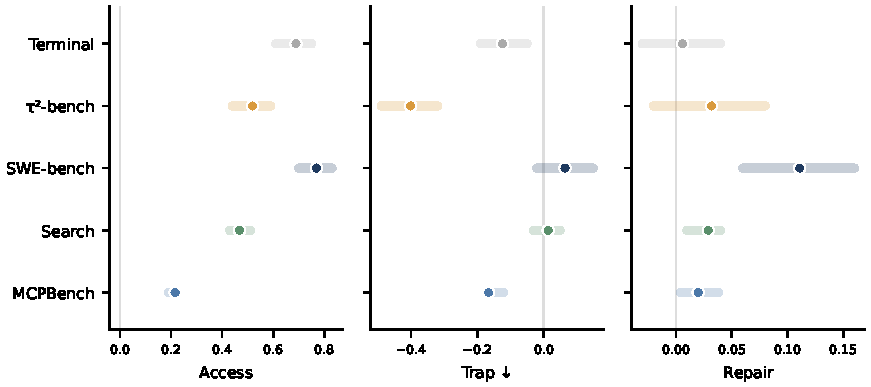
\includegraphics[width=\textwidth]{figures/fig_appendix_robustness.pdf}
\caption{Demand-sign robustness across hyperparameter sweeps. Dots show baseline values; shaded bars show the range across core-quantile, trap-quantile, Laplace-smoothing, diffusion, and mutual-$k$NN perturbations. All qualitative signs are stable except the borderline \terminal{} Trap sign under the largest mutual-$k$NN setting.}
\label{fig:robustness}
\end{figure*}

\subsection{Full Supply and Demand Tables}
\label{app:supply_demand_tables}

Tables~\ref{tab:model_profiles} and~\ref{tab:demand_vectors} give the exact numerical values underlying Figure~\ref{fig:supply_demand}.
Table~\ref{tab:model_profiles} reports model supply as task-centered residuals with task-bootstrap confidence intervals, while Table~\ref{tab:demand_vectors} reports benchmark demand as resolved-minus-failed contrasts (or the reward-weighted analogue for \mcp{}); positive Access and Repair indicate that high-outcome traffic uses those events more often, whereas negative Trap indicates stronger avoidance of low-outcome regions.

\begin{table*}[h]
\centering
\small
\setlength{\tabcolsep}{4pt}
\begin{tabular}{lccc}
\toprule
\textbf{Model} & \textbf{Access} & \textbf{Trap} & \textbf{Repair} \\
\midrule
DeepSeek-R1 & $-.022\;[-.043,-.001]$ & $+.012\;[-.010,+.035]$ & $+.007\;[-.007,+.020]$ \\
DeepSeek-V3.2 & $+.098\;[+.077,+.118]$ & $+.018\;[-.003,+.038]$ & $+.040\;[+.027,+.052]$ \\
Gemini-2.5-Flash & $-.022\;[-.040,-.004]$ & $-.024\;[-.041,-.006]$ & $-.017\;[-.025,-.009]$ \\
Qwen3-235B & $+.016\;[-.002,+.035]$ & $+.028\;[+.009,+.047]$ & $+.011\;[-.000,+.022]$ \\
Qwen3-Next & $-.092\;[-.116,-.067]$ & $-.042\;[-.067,-.017]$ & $-.049\;[-.058,-.039]$ \\
\bottomrule
\end{tabular}
\caption{Model supply profiles with 2,000 task-bootstrap $95\%$ CIs. Values are task-centered event residuals; because graph-valid task support differs by model, columns need not sum to zero exactly.}
\label{tab:model_profiles}
\end{table*}

\begin{table*}[h]
\centering
\small
\setlength{\tabcolsep}{4pt}
\begin{tabular}{lccc}
\toprule
\textbf{Benchmark} & \textbf{Access} & \textbf{Trap} & \textbf{Repair} \\
\midrule
\mcp{} & $+.216\;[+.182,+.249]$ & $-.166\;[-.199,-.130]$ & $+.020\;[-.004,+.042]$ \\
\searchb{} & $+.468\;[+.423,+.508]$ & $+.014\;[-.026,+.054]$ & $+.029\;[+.007,+.051]$ \\
\swe{} & $+.769\;[+.713,+.822]$ & $+.065\;[-.009,+.148]$ & $+.111\;[+.049,+.175]$ \\
\taub{} & $+.519\;[+.456,+.579]$ & $-.401\;[-.467,-.333]$ & $+.032\;[-.014,+.083]$ \\
\terminal{} & $+.689\;[+.637,+.738]$ & $-.124\;[-.177,-.067]$ & $+.006\;[-.024,+.038]$ \\
\bottomrule
\end{tabular}
\caption{Benchmark demand profiles with 2,000-bootstrap $95\%$ CIs. Negative Trap means high-outcome traffic avoids low-outcome regions.}
\label{tab:demand_vectors}
\end{table*}

\subsection{Additional Trap-Aware Recovery Details}
\label{app:trap_intervention_more}

\paragraph{Recovery arms.}
The three prefix-fork arms defined in \S\ref{sec:prefix_fork} separate two single-factor recovery routes.
\emph{Baseline} continues from the trigger snapshot at the baseline temperature $T{=}0.6$ with no inserted note.
\emph{Hot} switches the continuation to $T{=}0.9$, top-$p{=}0.95$ with no note, isolating the effect of increased sampling diversity.
\emph{Note} appends the diagnosis note at $T{=}0.6$, isolating the effect of evidence-grounded localization.

\begin{table}[h]
\centering
\small
\setlength{\tabcolsep}{5pt}
\begin{tabular}{ll}
\toprule
\textbf{Detector setting} & \textbf{Value} \\
\midrule
Trap similarity threshold & 0.35 \\
Trap--core margin & 0.03 \\
Warmup steps & 2 \\
Cooldown steps & 4 \\
Max triggers per rollout & 1 \\
Allowed intents & edit, submit \\
Observation-key gate & none \\
File-locality gate & require a \texttt{FILE\_PATH:*} cue \\
Rollout step budget & 30 total steps per arm \\
\bottomrule
\end{tabular}
\caption{Fixed detector and continuation settings used in the 500-instance \swe{} recovery study across all three providers.}
\label{tab:detector_hparams}
\end{table}

\paragraph{Conservative diagnosis note.}
The trap-side note is a fixed template populated at fire time.
The operative content is: re-read the failing test, traceback, or last database observation; localize to the smallest directly relevant function or read-only check; make one minimal change consistent with the evidence; and revise or discard the current edit/action if the evidence does not support it.
The slots are populated only from the agent's own per-step log: last command/action, last observation signal, implicated file or target keys, detector confidence, and a six-way family-level trap diagnosis.
No gold patch, verified-test list, or other oracle signal is used.

\paragraph{Tested instances.}
The main \method{}-guided recovery experiment uses the full 500-instance \swe{} Verified pool at seed $11$, covering all 12 \swe{} repositories that appear in the cx-cmu trajectory release: \texttt{django} ($231$), \texttt{sympy} ($75$), \texttt{sphinx-doc} ($44$), \texttt{scikit-learn} ($32$), \texttt{matplotlib} ($34$), \texttt{pytest-dev} ($19$), \texttt{astropy} ($22$), \texttt{pydata} ($22$), \texttt{pylint-dev} ($10$), \texttt{psf} ($8$), \texttt{mwaskom} ($2$), \texttt{pallets} ($1$).
The fired-subset analysis in the upper block of Table~\ref{tab:swe_4arm_intervention} uses each provider's own complete three-arm set ($n{=}196$ for GLM-5.1, $206$ for DeepSeek-V4-Pro, $214$ for Qwen3.6-35B-A3B); the common-fired analysis in the lower block restricts to the $96$ instances on which all three providers fire and produce a complete three-arm set.

\paragraph{Paired contrast statistics.}
Table~\ref{tab:swe_4arm_contrasts} reports the full set of paired contrasts that summarise Table~\ref{tab:swe_4arm_intervention}; the main-text intervention $p$-values refer to these same tests.
All confidence intervals use the cluster bootstrap with $10{,}000$ resamples clustered by instance id; $p$-values are one-sided paired-sign permutation against the alternative $\Delta > 0$.

\begin{table*}[h]
\centering
\small
\setlength{\tabcolsep}{5pt}
\renewcommand{\arraystretch}{1.05}
\begin{tabular}{llccc}
\toprule
\textbf{Subset / pool} & \textbf{Contrast} & \textbf{$\Delta$ (pp)} & \textbf{95\% CI (pp)} & \textbf{$p$} \\
\midrule
\multirow{2}{*}{GLM-5.1 ($n{=}196$)}        & Hot $-$ Baseline       & $+4.59$ & $[+0.0,+9.2]$  & $0.037$\,\checkmark \\
                                            & Note $-$ Baseline & $+1.53$ & $[-3.6,+6.6]$  & $0.348$ \\
\midrule
\multirow{2}{*}{DeepSeek-V4-Pro ($n{=}206$)}& Hot $-$ Baseline       & $+3.40$ & $[-1.5,+8.7]$  & $0.132$ \\
                                            & Note $-$ Baseline & $+0.97$ & $[-4.4,+6.3]$  & $0.428$ \\
\midrule
\multirow{2}{*}{Qwen3.6-35B-A3B ($n{=}214$)}& Hot $-$ Baseline       & $+1.40$ & $[-2.3,+5.1]$  & $0.332$ \\
                                            & Note $-$ Baseline & $+4.67$ & $[+0.0,+9.3]$ & $0.036$\,\checkmark \\
\midrule
\multirow{2}{*}{Per-provider fired pooled ($n{=}616$ cells)} & Hot $-$ Baseline       & $+3.08$ & $[+0.3,+5.9]$ & $0.016$\,\checkmark \\
                                            & Note $-$ Baseline & $+2.44$ & $[-0.6,+5.5]$  & $0.064^{\circ}$ \\
\midrule
\multirow{2}{*}{Common-fired pooled ($n{=}288$ cells)} & Hot $-$ Baseline       & $+3.82$ & $[+0.0,+8.0]$  & $0.045$\,\checkmark \\
                                            & Note $-$ Baseline & $+2.78$ & $[-2.1,+7.6]$  & $0.148$ \\
\bottomrule
\end{tabular}
\caption{Paired contrasts for Table~\ref{tab:swe_4arm_intervention}. Per-provider rows use each provider's own fired iids; the two pooled rows stack provider $\times$ iid cells (clustered by iid). \checkmark\,$p{<}0.05$; $^{\circ}$\,$p{<}0.10$.}
\label{tab:swe_4arm_contrasts}
\end{table*}

\subsection{Trap-Aware Intervention Case Studies}
\label{app:trap_case_studies}

\paragraph{Illustrative intervention cases.}
The following three cases separate a positive xarray example, a positive Django example, and a regression-style failure mode.

\paragraph{Case 1: \texttt{pydata\_\allowbreak{}\_xarray-4094}.}
The same trigger snapshot drives three qualitatively different recovery patterns across providers (Table~\ref{tab:case_xarray_4094}).
The detector fires while the agent is already reading \texttt{xarray/core/\allowbreak{}dataarray.py}, with trigger keys \texttt{ACTION:edit}, \texttt{CMD:sed}, \texttt{FILE\_PATH:xarray/core/\allowbreak{}dataarray.py}, and an earlier \texttt{ValueError} reproduction context.
Across providers, the raw assistant traces converge on the same local diagnosis: after selecting one variable from the stacked array, the stacked coordinate remains as a scalar coordinate, so later merging the per-variable arrays back into a dataset creates a coordinate conflict.
The divergence appears one refinement later.
Qwen3.6-35B-A3B under \emph{Baseline} and \emph{Hot} spends the post-trigger budget on reproduction and environment repair (missing \texttt{numpy}, then a \texttt{numpy} version mismatch) and never submits a patch.
Under \emph{Note}, it eventually reaches the right local fix idea and edits the key line to drop the stacked coordinate after \texttt{squeeze(drop=True)}, but the first version uses \texttt{drop\_vars(dim)} and then fails on the broader multi-dimensional round-trip test because the coordinate is not always present.
DeepSeek-V4-Pro shows a milder version of the same phenomenon: \emph{Baseline} reaches the right diagnosis but commits the brittle \texttt{drop(dim)} variant, whereas either \emph{Hot} or \emph{Note} is enough to move it to the safer \texttt{drop\_vars(dim,\allowbreak{} errors="ignore")} form.
GLM-5.1 is the easiest case: once triggered, both non-Baseline arms jump directly to that safe one-line fix.

\begin{table}[h]
\centering
\scriptsize
\setlength{\tabcolsep}{4pt}
\begin{tabular}{lccc}
\toprule
\textbf{Provider} & \textbf{Baseline} & \textbf{Hot} & \textbf{Note} \\
\midrule
GLM-5.1            & no patch          & \cellcolor{bestcolor}\checkmark\,(572\,ch) & \cellcolor{bestcolor}\checkmark\,(572\,ch) \\
DeepSeek-V4-Pro    & \texttimes (550\,ch) & \cellcolor{bestcolor}\checkmark\,(572\,ch) & \cellcolor{bestcolor}\checkmark\,(572\,ch) \\
Qwen3.6-35B-A3B    & no patch          & no patch & \texttimes (555\,ch) \\
\bottomrule
\end{tabular}
\caption{\texttt{pydata\_\allowbreak{}\_xarray-4094} per-arm outcomes. \checkmark\ marks resolved; \texttimes\ marks a submitted patch that fails the verified tests; ``no patch'' marks an empty submission. Parentheses show patch length in characters.}
\label{tab:case_xarray_4094}
\end{table}

\paragraph{Case 2: \texttt{django\_\allowbreak{}\_django-13128}.}
The trigger fires later in the rollout, after the agent has already narrowed the bug to \texttt{django/db/models/\allowbreak{}expressions.py} and is inspecting \texttt{CombinedExpression} with an \texttt{OBS:error} context (Table~\ref{tab:case_django_13128}).
The trap here is not a wrong first diagnosis but a low-yield validation loop.
In the GLM-5.1 \emph{Baseline} trace, the model states the correct diagnosis almost immediately in its own scratch reasoning: subtracting two temporal fields is being inferred as \texttt{DateTimeField} when it should produce \texttt{DurationField}.
But the baseline rollout then burns budget on environment setup and brittle ad-hoc probes, repeatedly re-deriving the same explanation without committing a final patch.
\emph{Hot} and \emph{Note} both shorten that loop.
The successful GLM arms add a narrow \texttt{\_resolve\_\allowbreak{}output\_field()} override directly to \texttt{CombinedExpression}, then fix one subtle bug exposed by a direct probe: comparing field \emph{instances} with \texttt{==} is too strict, so the final patch compares field types / internal types and returns \texttt{fields.\allowbreak{}DurationField()} only for temporal subtraction.
The \emph{Note} arm is especially illustrative: after trigger it stays anchored to the smallest relevant region---\texttt{CombinedExpression} and the temporal-subtraction tests---rather than relaxing the global mixed-type logic elsewhere in \texttt{BaseExpression}.
DeepSeek-V4-Pro shows the complementary provider-specific pattern on the same instance.
Only \emph{Hot} reaches a submitted fix; the \emph{Note} arm remains in the expression-tree / test-harness analysis loop and ends with an empty submission, matching the aggregate result that this provider benefits mainly from extra sampling diversity rather than the diagnosis note itself.

\begin{table}[h]
\centering
\scriptsize
\setlength{\tabcolsep}{4pt}
\begin{tabular}{lccc}
\toprule
\textbf{Provider} & \textbf{Baseline} & \textbf{Hot} & \textbf{Note} \\
\midrule
GLM-5.1         & no patch & \cellcolor{bestcolor}\checkmark\,(1057\,ch) & \cellcolor{bestcolor}\checkmark\,(1001\,ch) \\
DeepSeek-V4-Pro & no patch & \cellcolor{bestcolor}\checkmark\,(1175\,ch) & no patch \\
\bottomrule
\end{tabular}
\caption{\texttt{django\_\allowbreak{}\_django-13128} per-arm outcomes for the two providers discussed in the text. Parentheses show patch length in characters.}
\label{tab:case_django_13128}
\end{table}

\paragraph{Case 3: failure mode on \texttt{django\_\allowbreak{}\_django-14311}.}
The same framework can also hurt performance when the note over-focuses the continuation on an overly narrow local pattern.
On \texttt{django\_\allowbreak{}\_django-14311}, the trigger fires while GLM-5.1 is already inspecting \texttt{tests/utils\_tests/\allowbreak{}test\_autoreload.py}, with trigger keys anchored to an edit candidate in the autoreload path and an earlier \texttt{RuntimeError} context.
All three arms correctly identify the broad bug family: \texttt{get\_child\_\allowbreak{}arguments()} should reconstruct the \texttt{-m} target from \texttt{\_\_\allowbreak{}main\_\_.\allowbreak{}\_\_spec\_\_}.
But the Note arm overcommits to the immediately visible package-with-\texttt{\_\_\allowbreak{}main\_\_} example from \texttt{utils\_tests.\allowbreak{}test\_module}.
It rewrites the logic to always use \texttt{\_\_\allowbreak{}spec\_\_.name.\allowbreak{}removesuffix('.\_\_\allowbreak{}main\_\_')}, which fixes the package case but breaks the non-package module case and regresses three previously passing tests.
By contrast, the successful \emph{Baseline} arm makes the minimal string replacement \texttt{name.\allowbreak{}replace('.\_\_\allowbreak{}main\_\_', '')}, and the successful \emph{Hot} arm reaches the same fix with a slightly different edit path.
This is a concrete example of a trap-aware note becoming too prescriptive: it improves localization, but can also bias the model toward an over-specialized repair if the visible trigger context is only one branch of the full behavioral contract.

\begin{table}[h]
\centering
\scriptsize
\setlength{\tabcolsep}{4pt}
\begin{tabular}{lccc}
\toprule
\textbf{Provider} & \textbf{Baseline} & \textbf{Hot} & \textbf{Note} \\
\midrule
GLM-5.1 & \checkmark\,(694\,ch) & \checkmark\,(953\,ch) & \texttimes\,(852\,ch) \\
\bottomrule
\end{tabular}
\caption{A regression-style intervention case. On \texttt{django\_\allowbreak{}\_django-14311}, the Note arm fails \texttt{test\_run\_as\_non\_django\_\allowbreak{}module\_non\_package} and three pass-to-pass autoreload tests, while the other two arms resolve the instance.}
\label{tab:case_failure_django_14311}
\end{table}

\subsection{Agent Framework and Recovery Templates}
\label{app:templates}

The \swe{} continuation agent is a single-tool bash agent.
We reproduce here the templates that fully specify what the agent sees on every step and what each arm injects: the system prompt that fixes the response format, the issue-statement user message, the observation wrapper used after every command, and the 5-block diagnosis-note template that the \emph{Note} arm injects at the trigger step (with the \emph{Baseline} and \emph{Hot} arms injecting nothing).

\paragraph{System prompt.}
Used as the first message of every rollout, on every arm.

\begin{tcolorbox}[colback=gray!10, colframe=gray!50, boxrule=0.5pt, breakable]
\tiny
\begin{Verbatim}[breaklines,breakanywhere]
You are a software engineer tasked with solving a GitHub issue. You have access to a bash shell to explore the repository, understand the codebase, locate the relevant code, and make the necessary changes to fix the issue.

## Response Format

Every response must contain exactly TWO sections:

1. **THOUGHT**: Your reasoning about what to do next. Analyze the problem, plan your approach, and explain your next step.

2. **ACTION**: A single bash command to execute. This must be wrapped in a bash code block.

Example response:

THOUGHT:
I need to find the file that contains the buggy function.

ACTION:
```bash
find . -type f -name "*.py" | xargs grep -l "def process_data"
```

## Important Rules

- Each response must contain exactly ONE bash command in the ACTION section.
- To submit your solution when done, use the special command:
  ```bash
  submit
  ```
- Do NOT run interactive commands (vim, nano, python REPL, etc.).
- Do NOT use `git push` or modify remote state.
- Keep your changes minimal and focused on the issue.
- Always verify your fix with relevant tests before submitting.
- If you need to edit a file, use `sed`, `awk`, or heredoc redirects.
- If a command produces too much output, pipe through `head` or `tail`.
\end{Verbatim}
\end{tcolorbox}

\paragraph{Initial user message.}
Inserted once at step $0$ to communicate the GitHub issue. The placeholder \verb|{problem_statement}| is filled with the verbatim \swe{} Verified \texttt{problem\_statement} field.

\begin{tcolorbox}[colback=gray!10, colframe=gray!50, boxrule=0.5pt, breakable]
\tiny
\begin{Verbatim}[breaklines,breakanywhere]
Here is the GitHub issue to solve:

<issue>
{problem_statement}
</issue>

You are in the repository root. The repository has already been checked out to the correct commit. Explore the repo, understand the issue, make the fix, and run tests to verify. When you are confident your fix is correct, use the `submit` command.
\end{Verbatim}
\end{tcolorbox}

\paragraph{Per-step observation wrapper.}
After every \texttt{ACTION} bash command, the harness executes it inside the docker workspace and returns the (truncated) combined stdout/stderr to the agent as a user message wrapped in:

\begin{tcolorbox}[colback=gray!10, colframe=gray!50, boxrule=0.5pt]
\tiny
\begin{Verbatim}[breaklines,breakanywhere]
OBSERVATION:
{observation}
\end{Verbatim}
\end{tcolorbox}

\paragraph{Trap-diagnosis note (Note arm).}
At the trigger step both \textsc{Note}-on arms inject the following message as a user message immediately after the last observation, before the agent's next \texttt{THOUGHT}/\texttt{ACTION} turn. The header marks the message as internal; the five slots \verb|{ctx_command}|, \verb|{ctx_signal}|, \verb|{ctx_files}|, \verb|{ctx_confidence}|, \verb|{ctx_trap_pattern}| are populated only from the agent's own per-step log and a per-pattern diagnosis sidecar; no gold-patch or verified-test information is used.

\begin{tcolorbox}[colback=gray!10, colframe=gray!50, boxrule=0.5pt, breakable]
\tiny
\begin{Verbatim}[breaklines,breakanywhere]
[INTERNAL DIAGNOSTIC -- not visible to graders]
A trajectory pattern previously associated with low task-resolution rates fired at this step. Concretely:

  - Last command: {ctx_command}
  - Last error/test signal: {ctx_signal}
  - File(s) touched in this region: {ctx_files}
  - Detector confidence (trap similarity): {ctx_confidence}

  Trap pattern (from prior failed trajectories with this signature):
  {ctx_trap_pattern}

Before continuing:
  1. Re-read the failing test/traceback for the specific assertion or unexpected value (do not rely on memory of earlier steps).
  2. Localize to the smallest function or class implicated by that evidence, in the file(s) above.
  3. Propose ONE minimal change consistent with the evidence; do not rewrite unrelated code.
  4. Run the narrowest relevant test or check before submitting.
  5. If your current patch is not supported by the error/test evidence, revise or discard it.

Respond in the normal THOUGHT / ACTION format with exactly one bash command.
\end{Verbatim}
\end{tcolorbox}

\paragraph{Slot filling.}
At trigger time the slots are populated from the agent's own per-step record (no oracle signal):
\verb|{ctx_command}| is the most recent \texttt{ACTION} bash command, truncated to $200$ characters;
\verb|{ctx_signal}| is the most recent observation passed through a fixed regular-expression family for traceback / pytest / syntax / import / missing-file / timeout cues, truncated to $300$ characters;
\verb|{ctx_files}| is the top-$3$ file paths from the trigger key set (only files the agent itself has opened in its own commands);
\verb|{ctx_confidence}| is the trap similarity score $\mathrm{sim}_{\mathrm{trap}}$ formatted to two decimals;
\verb|{ctx_trap_pattern}| is the family-level diagnosis string for the matched trap pattern (one of six pre-specified families), read from a sidecar JSON keyed on the trap key-set fingerprint.
The \emph{Baseline} and \emph{Hot} arms inject nothing at the trigger step; the conversation proceeds directly from the trigger observation to the agent's next \texttt{THOUGHT}/\texttt{ACTION} turn at the arm's continuation temperature.

\section{Algorithmic Details}
\label{app:algos}


\subsection{Signature Key Alphabet}
\label{app:keys}

A step's symbolic key set $K_i$ contains keys from the channels in Table~\ref{tab:keys}.
Keys are case-sensitive and prefix-tagged, so different channels never collide in the IDF dictionary.
Observation keys are produced by fixed regular-expression families over the first $2{,}000$ characters of the tool response; the families include error, traceback, test pass/fail, syntax error, import error, missing file, permission error, timeout, and explicit success messages.
The search-specific keys (\texttt{URL\_DOMAIN}, \texttt{QUERY\_NOVELTY}, \texttt{EVIDENCE\_COUNT}) are pre-specified from the search tool-call/result format, not selected from outcome inspection.

\begin{table}[h]
\centering
\scriptsize
\setlength{\tabcolsep}{3pt}
\begin{tabularx}{\linewidth}{lX}
\toprule
\textbf{Channel} & \textbf{Information captured} \\
\midrule
Tool name & Tool or API name after benchmark-specific prefix stripping. \\
Action type & Coarse action class such as bash, edit, read, search, submit, or other. \\
Command class & Shell-command families such as pytest, grep, cat, sed, python, and git. \\
Observation pattern & Error, pass/fail, timeout, missing-file, and success cues. \\
File cue & Last path components and file extensions mentioned in the action. \\
Temporal phase & Early, middle, or late third of the rollout. \\
Search-only & URL/result domain (eTLD$+1$), query novelty (new/refine/repeat), and cumulative distinct-domain count buckets. \\
\bottomrule
\end{tabularx}
\caption{Compact signature key alphabet used by the signature extractor.}
\label{tab:keys}
\end{table}


\subsection{Reward Field, Core and Trap Masks, Block Quotient Graph}
\label{app:roles_math}

The \emph{block quotient graph} $G_B=(B,E_B)$ has one node per non-trivial BCC and an undirected edge $(b,b')\in E_B$ weighted by the number of slices shared between the two blocks.
Edge weights are row-stochastically normalized into a transition matrix $P_B$, and the teleport-$\alpha$ diffusion update is
\begin{equation}
v^{(t+1)} = \alpha\, P_B^{\top} v^{(t)} + (1-\alpha)\, s,
\label{eq:diffuse}
\end{equation}
where $\mathcal{R}_b$ is the set of rollouts visiting block $b$, and the seed $s_b=\hat\mu_b-\bar y_t$ is the Laplace-smoothed excess outcome of block $b$ relative to the task average, with $\hat\mu_b=(\sum_{r\in\mathcal{R}_b} y_r+\tfrac{1}{2})/(|\mathcal{R}_b|+1)$.
We iterate Eq.~\ref{eq:diffuse} for $T=24$ steps with $\alpha=0.65$ and L$\infty$-normalize to $[-1,1]$.
Let $Q^+_{.75}$ be the 75th percentile of positive field values and $Q^-_{.25}$ the 25th percentile of negative field values.
The role overlays used in the main text are then:
\begin{align}
C_t &= \{b:\, v^{(T)}_b>0 \;\wedge\; v^{(T)}_b\geq Q^+_{.75}\}, \\
B_t &= \{b:\, v^{(T)}_b<0 \;\wedge\; v^{(T)}_b\leq Q^-_{.25}\}.
\end{align}
Note that $B_t$ is a direct bottom-quartile mask of the negative diffusion field, which avoids a circularity between the trap definition and the $R_r$ event.
Articulation points remain useful for graph visualization and the RQ1 sanity annotation, but they are not used as a main rollout event or as a recovery target.
